\documentclass[11pt]{scrartcl}
\usepackage[utf8]{inputenc}
\usepackage{amsmath, amssymb}
\usepackage{natbib}
\usepackage{graphicx}
\usepackage{fullpage}
\usepackage{subcaption}
\usepackage{booktabs}

\usepackage{tikz}
\usetikzlibrary{bayesnet}

\newcommand{\ie}{\textit{i.e.}}
\newcommand{\cat}{\text{Cat}}
\newcommand{\thetaold}{\theta^{t}}
\newcommand{\Cat}{\text{Cat}}

\title{Unsupervised Lexicon Annotation using Expectation Maximization} 
\author{Jorn Peters\\\small{jornpeters@gmail.com} \and Bram van den Akker\\\small{contact@bramvandenakker.nl}}

\begin{document}

\maketitle

\abstract{In this paper a subset of the work
in~\cite{rooth1999inducing} is reproduced. Specifically, a model for
slot annotations and sub-categorizations are presented and
evaluated. Both models are inferred using Expectation Maximization
using data obtained from parsing the Penn Tree Bank and British News
corpora. An analysis of the obtained model is given. }

\section{Introduction} % Bram
Finding the relation between verbs and their arguments is a classic problem in lexical semantics. In 1993, Levin \cite{levin1993english} argued that semantically coherent classes could be created by examining their context which can then be used to disambiguate the verbs. According to \cite{lapata2004verb}, these classes have various limitations for use in computational models. In their study, they create a simple statistical model for verb class ambiguity extending Levin's classes. This study covers two methods for slot annotation and
sub-categorization on annotated data. The first part is a reproduction of the work presented in~\cite{rooth1999inducing}, where both a slot annotation and
sub-categorization are induced using the
Expectation Maximization~\cite{dempster1977maximum} (EM). More specifically, a latent clustering model is used to infer
Parser~\cite{klein2003accurate}. The second part of the paper describes an alternative method for sub-categorization that uses Variational Autoencoders (VAE) with the word embeddings creating from the verbs and nouns. The rest of this paper is as follows:
clusters for verb-noun pairs that were extracted using the Stanford
In section two the clustering approach is presented, in Section 2.1
and 2.2 the two models are described. Section 3 the evaluation method
is outlined, results are discussed in Section 4 and a conclusion is
given in Section 5. % Laatste gedeelte nodig? Of was het gewoon om tekst te vullen? 

\section{EM Clustering} % Jorn
Following~\cite{rooth1999inducing}
Expectation-Maximization~\cite{dempster1977maximum} (EM) is used to
infer latent classes of verb-noun pairs consisting of a verb head, grammatical relation and noun filler head. The verb-noun pairs are
extracted from the Penn Tree Bank (PTB) and British News (BTC) corpora
using the Stanford parser\footnote{The extracted verb-noun pairs were
provided as part of the Unsupervised Language Learning course at the
University of Amsterdam.}~\cite{klein2003accurate}.  The inferred
classes can be interpreted as automatically induced slot annotations
of sub-categorizations frames.

% Why use EM
EM is a well understood iterative algorithm that maximizes the
marginal log-likelihood of the observed data of a parametric model in
the case were some variables of the model are unobserved or
\textit{latent}. Using EM, the marginal log-likelihood monotonically
increases after each iteration. Hence, it is a very stable algorithm
which will convergence with probability one, given that it run for
enough iterations. For the present case, EM provides a well-defined
framework that is easy to derive and fast to execute.

% Briefly explain procedure
The EM algorithm consists of two steps, the expectation step (E-step)
and the maximization step (M-step). In th E-step the function
$\mathcal{Q}(\theta|\theta^t) =
\mathbb{E}_{p_{\theta^t}(Z|X)}[\log p_{\theta}(X, Z)]$ is evaluated. Here 
$X$ is the set of observed variables, $Z$ is the set of latent
variables, and $\theta$ is the set of model parameters. The E-step if
followed by the M-step in which the parameters are optimized, \ie,
\[
  \theta^{t+1} = \arg\max_{\theta} \mathcal{Q}(\theta | \theta^t).
\]
These two steps are performed in an iterative manner, after each
application both the E-step and the M-step the log-likelihood
monotonically increases, making EM a very well behaved algorithm. The
main disadvantage of EM is that it is not guaranteed to converge to
a global maximum, making multiple runs a necessity.

% Setup model prereqs
For the rest of this paper, the following notation is used. Let $V$
denote the set of all verbs in the dataset, $N$
the set of all nouns, $\mathcal{Y} = \{(v_1, n_1), \ldots, (v_M,
n_M)\}$ the set of all verb-noun pairs available in the data set, where
$v_i \in V$ and $n_i \in N$. In the following sections, the specific
models used for automatic induction are discusses. More specifically,
in Section~\ref{sec:verbclasses} the model for automatic induction of
slot annotations is described and in Section~\ref{sec:nounclasses} the
model for deducing sub-categorizations is presented.

\begin{figure}
\centering
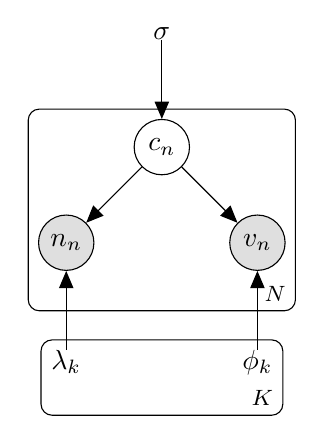
\begin{tikzpicture}

  % Define nodes
  \node[latent] (cn) {$c_n$};
  \node[const, above=of cn] (sigma) {$\sigma$};
  \node[obs, below right=of cn] (vn) {$v_n$};
  \node[obs, below left=of cn] (nn) {$n_n$};
  \node[const, below=of nn] (lamb) {$\lambda_k$};
  \node[const, below=of vn] (phi) {$\phi_k$};
  % \node[latent, above=of y, xshift=-1.2cm] (w) {$\mathbf{w}$};
  % \node[latent, above=of y, xshift=1.2cm]  (x) {$\mathbf{x}$};
  % \node[latent, right=2cm of y]            (t) {$\tau$};

  % Connect the nodes
  \edge {cn} {vn, nn} ; 
  \edge {sigma} {cn} ; 
  \edge{phi}{vn};
  \edge{lamb}{nn};

  % Plates
  \plate {yx} {(cn)(vn)(nn)} {$N$} ;
  \plate {k} {(phi)(lamb)} {$K$} ;
  % \plate {} {(w)(y)(yx.north west)(yx.south west)} {$M$} ;

\end{tikzpicture}
\caption{Graphical model of clustering model. $N$ denotes the total
number of pairs in teh dataset. $c_n$, $v_n$, and $n_n$ denote the
$n$th class, verb and noun, respectively. In total $K$ classes are
considered.}
\label{fig:graphmodel}
\end{figure}


\subsection{Slot Annotation Model} % Jorn
\label{sec:verbclasses}
In this section a model is presented that induces a distribution of
latent clusters for each verb-noun pair. These clusters can be
used for the induction of slot annotations. Moreover, for each cluster a distribution over verbs and a distribution of nouns. The
model is defined as follows:
\begin{align*}
  p(\mathcal{Y})
  &= \prod_{m=1}^M \sum_{k=1}^K p(k)p(v_m|k)p(n_m|k) \\
  &= \prod_{m=1}^M \sum_{k=1}^K \Cat(k|\sigma)\Cat(v_m|\phi^k)\Cat(n_m|\lambda^k) \\
\end{align*}
where $\sigma, \phi^k, \lambda^K$ for $k=1,\ldots,K$ are the
parameters of this model, for $\sigma \in \mathbb{R}_{\ge 0}^K$ $\phi^K \in
\mathbb{R}_+^{|V|}$, and $\lambda^k \in \mathbb{R}_+^{|N|}$. All
parameter vectors are constrained to sum to one. Note that the verbs
and nouns in each pair are independent but become dependent once the
class is observed. The graphical model for this model is depicted in
Figure~\ref{fig:graphmodel}. Since this is a latent variable model, EM
is used to find the maximum likelihood estimate of the parameters of
the model.

To perform the EM algorithm, the update equations/steps are derived. A
detailed derivation is included in Appendix~\ref{sec:part1}, and here
the steps are stated. To evaluate the expectation of the complete
log-likelihood under the distribution of the latent variables
conditioned on the observed variables, the conditional probability
\[
  p(c | v_m, n_m , \theta^t) = \frac{\sigma^t_c \phi^{c,t}_{v_m}\lambda^{c, t}_{n_m}} {\sum_{k=1}^K \sigma^t_k \phi^{k,t}_{v_m}\lambda^{k, t}_{n_m}}
\]
is evaluated. In the M-step the following updates are performed:
 \begin{align*}
     \sigma_k^{t+1} &= \frac{1}{M} \sum_{m=1}^M p(k|v_m, n_m), \\
     \phi_v^{k,t+1} &= \frac{\sum_{m=1}^M [v_m = v] p(k|v_m, n_m, \thetaold)}
                     {\sum_{m=1}^M p(k|v_m, n_m, \thetaold)}, \\
     \lambda_n^{k,t+1} &= \frac{\sum_{m=1}^M [n_m = n] p(k|v_m, n_m, \thetaold)}
                     {\sum_{m=1}^M p(k|v_m, n_m, \thetaold)}.
 \end{align*}
 After running the EM algorithm for a sufficient number of iterations
 (\textit{e.g.}, such that the increase in log-likelihood becomes small)
 a distribution over classes is inferred for each verb-noun pair, and
 for each class a distribution over nouns and a distribution over
 verbs is available.

\subsection{Sub-Categorization Model} % Jorn
\label{sec:nounclasses}
The sub-categorization model defines a distribution over nouns for a
specific intransitive verb. That is, given intransitive verb $v_i$,
the set $N_{v_i} = \{n^i_1, \ldots\}$ of nouns that act as the subject
of $v_i$ is collected. Then, a distributions over these nouns is
inferred given a latent class model $p_{LC}(\cdot|\cdot)$ for nouns, \ie,
\begin{align*}
  p(N_{v_i}) &= \prod_{j=1}^{|N_{v_i}|} \sum_{k=1}^K q(k)p_{LC}(n^i_j|k) \\
            &= \prod_{j=1}^{|N_{v_i}|} \sum_{k=1}^K \Cat(k|\theta)\Cat(n^i_j|\lambda^k) \\
            &= \prod_{j=1}^{|N_{v_i}|} \sum_{k=1}^K \theta_k \lambda^k_{n^i_j}
\end{align*}
where $q(k)$ defines the probability of the class $k$ (using a
different model than that used in the previous section), and the
latent class model for nouns that was inferred using the model in the
previous section is used. Then following the typical EM steps, in the E-step
\begin{align*}
    p(k|n^i_j, \theta^t) &= \frac{p(k)p(n^i_j|k)}{\sum_{k'=1}^K  p(k')p(n^i_j|k')} \\
               &= \frac{\theta^t_{k}\lambda^{k}_{n^i_j}}{\sum_{k'=1}^K  \theta^t_{k'}\lambda^{k'}_{n^i_j}}
\end{align*}
is evaluated for all $k = 1,\ldots,K$ and $n^i_j \in N_{v_i}$. Since
the only parameter of this model (as the noun latent class model is
given) is $\theta$, there is only a single update equation, \ie,
\begin{align*}
  \theta^t_k = \frac{1}{N} \sum_{i=1}^N p(k | n^i_j, \theta^t)
\end{align*}
Since the derivation of these update equations are essentially the
same as of those of the model in the previous section, no explicit
derivation of the equations are included in this paper or the
appendix.

\section{EM Evaluation} % Jorn
The slot annotation model is evaluated using an evaluation scheme
devised in~\cite{rooth1999inducing}. The sub-categorization model is
evaluation by inspection. That is, the high probability nouns for each
cluster are inspected, it is then expected that for each cluster the
high probability nouns are similar, \ie, can be used in similar
situations.

The slot annotation model is evaluated using an experiment that tests
if nouns related to a verb (\ie, occur in the data set) get higher
conditional probability than that same noun related to a random
verb. More specifically, 3000 verb-noun $(v, n)$ pairs are samples
from the data set. For each samples pair another verb $v'$ is sampled
such that $(v', n)$ does not occur in the data set, resulting in the
triples $(v, n , v')$. Each triple for which one element occurs less
than 30 or more than 3000 times in the data set are discarded. All
remaining triples form the test set and all occurrences of $(v, n)$
are removed from the training set. This procedure resulted in 1285
triples in the test set. Then the accuracy of the model is computed as
the percentage of triples for which $p(n|v) \ge p(n|v')$, where
\[
  p(n|v) = \frac{p(n, v)}{p(v)} =
  \frac{\sum_{k=1}^k p(k)p(v|k)p(n|k)}{\sum_{n=1}^{|N|}\sum_{k=1}^K p(k)p(v|k)p(n|k)}.
\]
The results are presented in Section~\ref{sec:results}.

\section{EM Results} % Jorn & Bram
\label{sec:results}
Figure~\ref{fig:accuracy} shows the accuracy results for the slot
annotation model. The results are similar to those observed
in~\cite{rooth1999inducing}. Namely, first the accuracy increases when
the number of clusters is increased, but at some point the accuracy
decreases again. In contrast to~\cite{rooth1999inducing}, the numbers
of clusters for which the best result is obtained is higher, \ie,
approximately 75 compared to approximately 35\footnote{approximately,
since the model was not run for all number of clusters.}. Moreover,
the best accuracy obtained in the present study is lower than that
obtained by~\cite{rooth1999inducing}. These differences can be
explained by the fact that for the present study a more advanced
parser was used to extract the pairs. Although this does not
necessarily make the tasks harder, it is possible that the current
parser is better at extracting harder pairs. However, a definitive
statement on this needs more work.

\begin{figure}
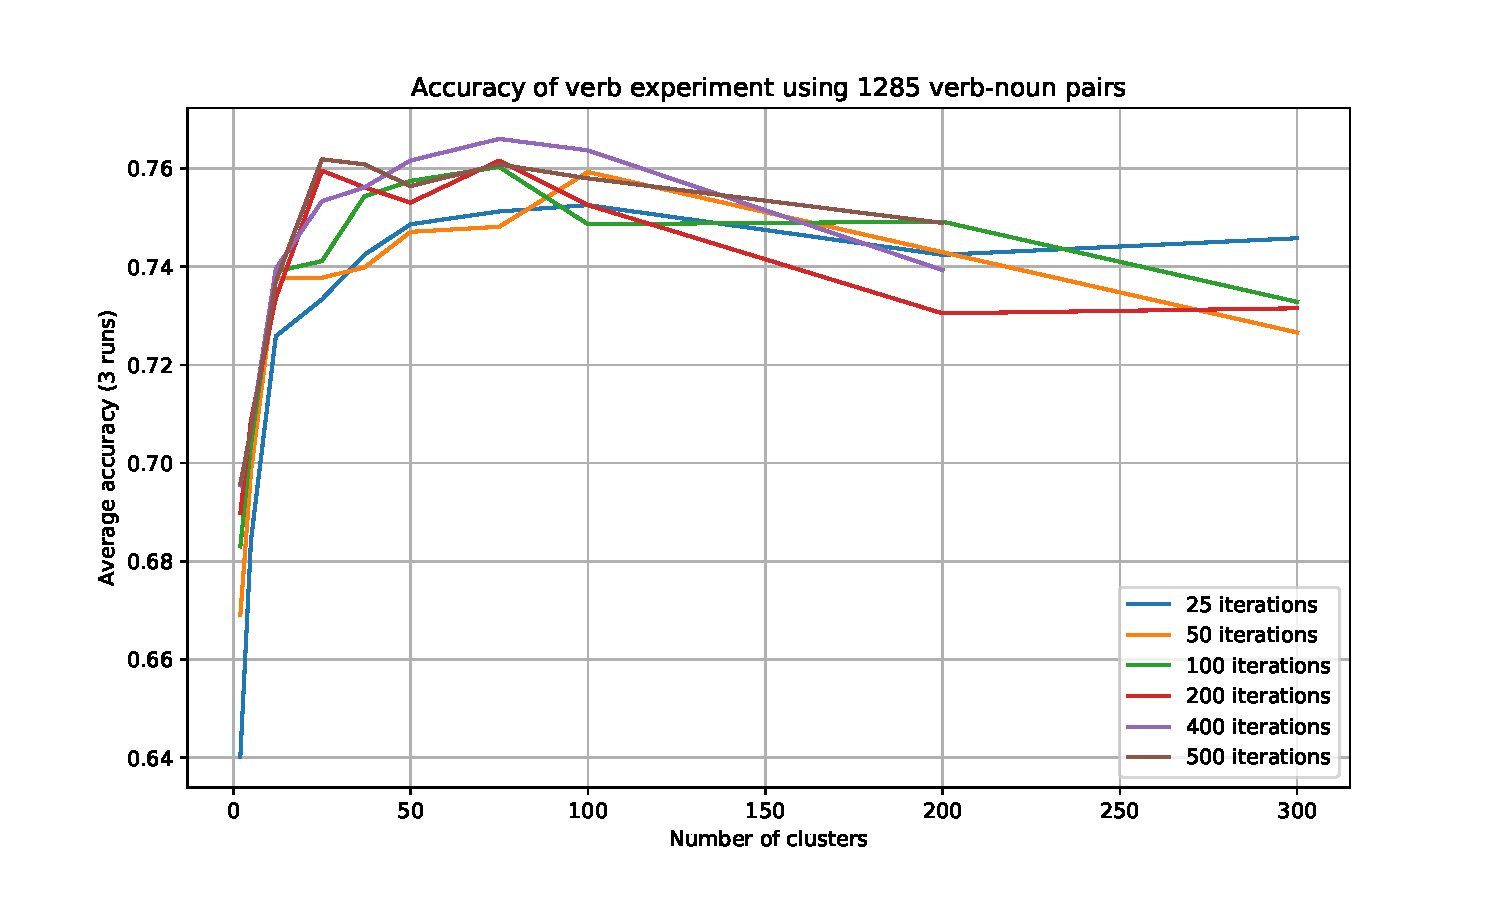
\includegraphics[width=\textwidth]{slotresults.pdf}
\caption{Accuracy averaged over three runs of different parameters
settings (maximum number of iterations, numbers of clusters). Note
that the results for 400 and 500 iterations for $>$ 200 clusters are
missing due to memory requirements.}
\label{fig:accuracy}
\end{figure}

The slot annotation model is set up such that elements of a verb-noun
pair are dependent given the class. Hence, it is expected that given a
class, the high probability verbs and nouns will have high probability
of occurring as a pair in the data set. Figure~\ref{fig:kde} shows
density plots for verb noun pairs occurring in the data set for the
top 1000 verbs and nouns in four different classes. This clearly shows
the top nouns and top verbs often occur as pairs in the data set,
whereas the nouns and verbs with lower probability occur less often to
never in the data set. Note that although here only four classes are
shown, this pattern is similar for all classes. However, apart from
the top $\sim 50$ classes different patterns emerge for different
classes. For example, class 6 has a low number of nouns occurring with
a high number of verbs and class 10 show the exact opposite pattern.
Table~\ref{table:top10} shows the top-10 nouns and verbs for these
classes, the difference in pair patterns is easily explained based on
this. Class 6 gives high probability to nouns referring to people,
these are used with many different verbs, moreover, class 24 give high
probability to verbs such as \textit{have, had has, \ldots}, which are
also used in many situations, combined with many different nouns.

\begin{figure}

  \begin{subfigure}[b]{0.5\textwidth}
    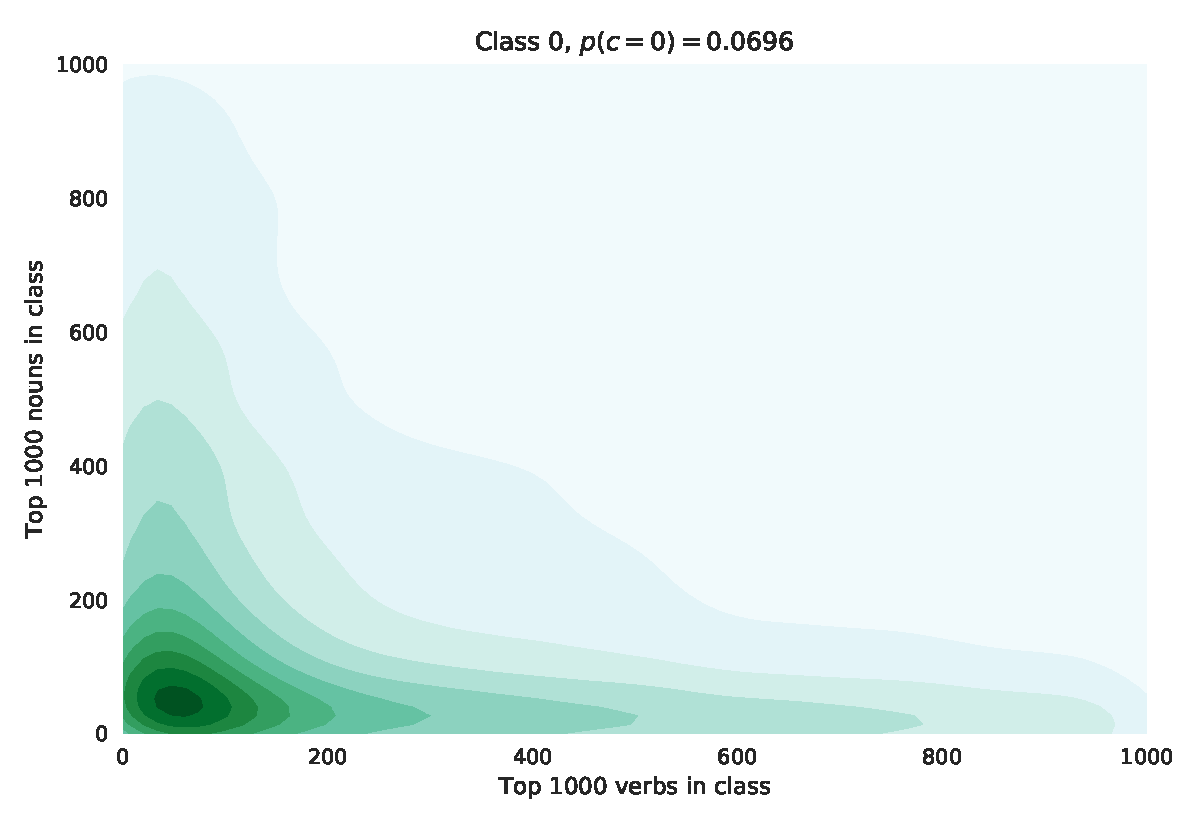
\includegraphics[width=\textwidth]{class_0.pdf}
  \end{subfigure}
  \begin{subfigure}[b]{0.5\textwidth}
    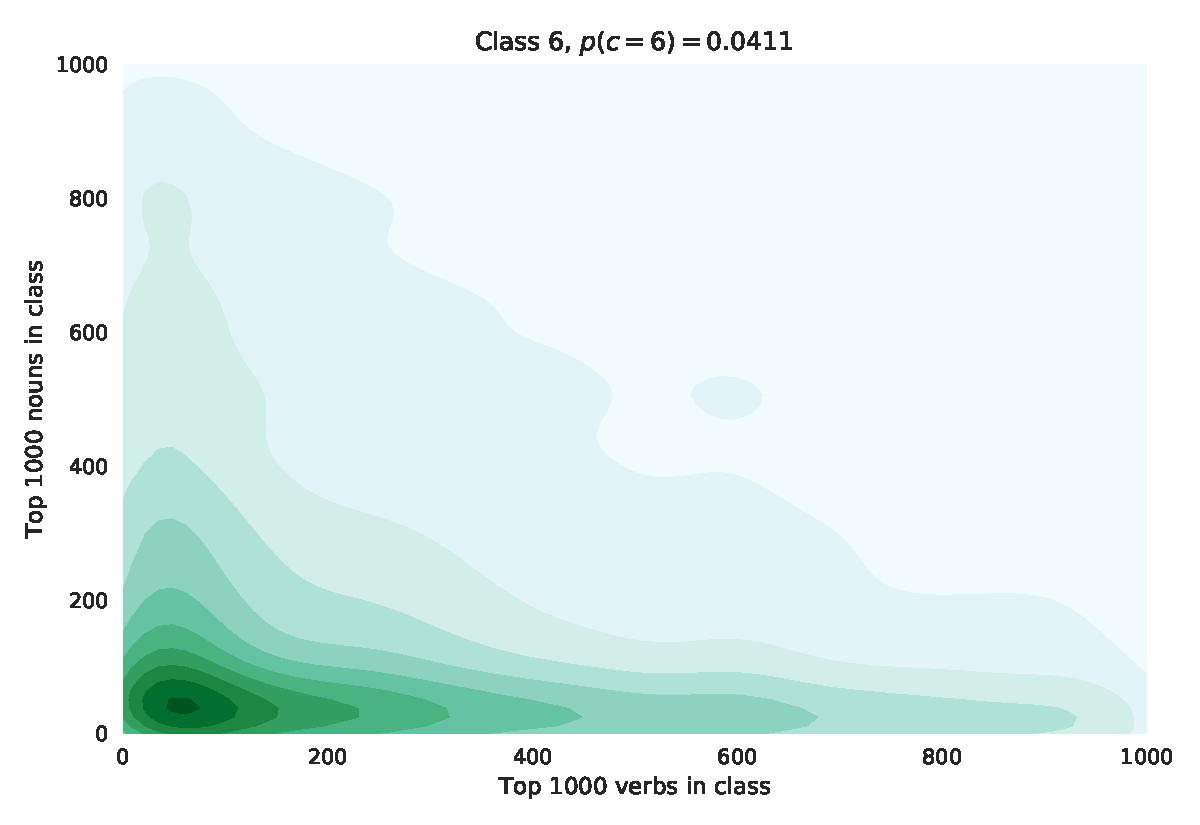
\includegraphics[width=\textwidth]{class_6.pdf}
  \end{subfigure}

  \begin{subfigure}[b]{0.5\textwidth}
    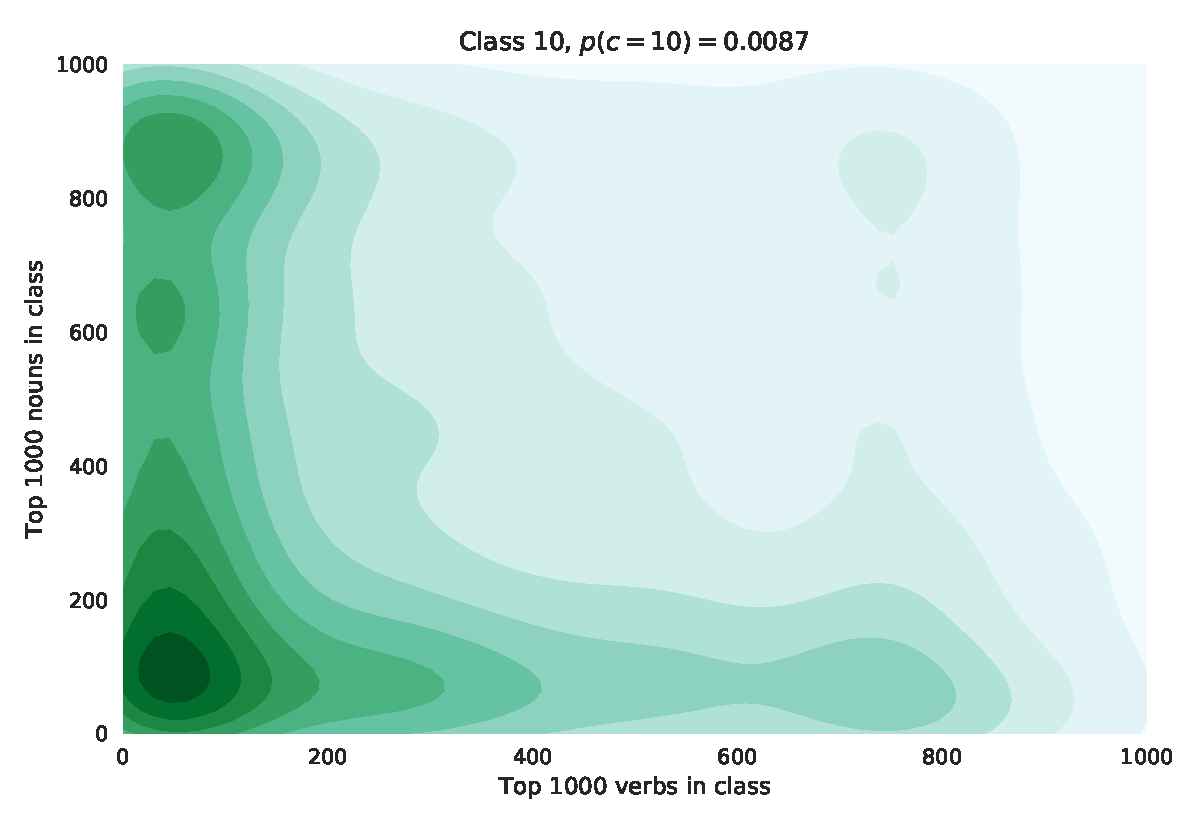
\includegraphics[width=\textwidth]{class_10.pdf}
  \end{subfigure}
  \begin{subfigure}[b]{0.5\textwidth}
    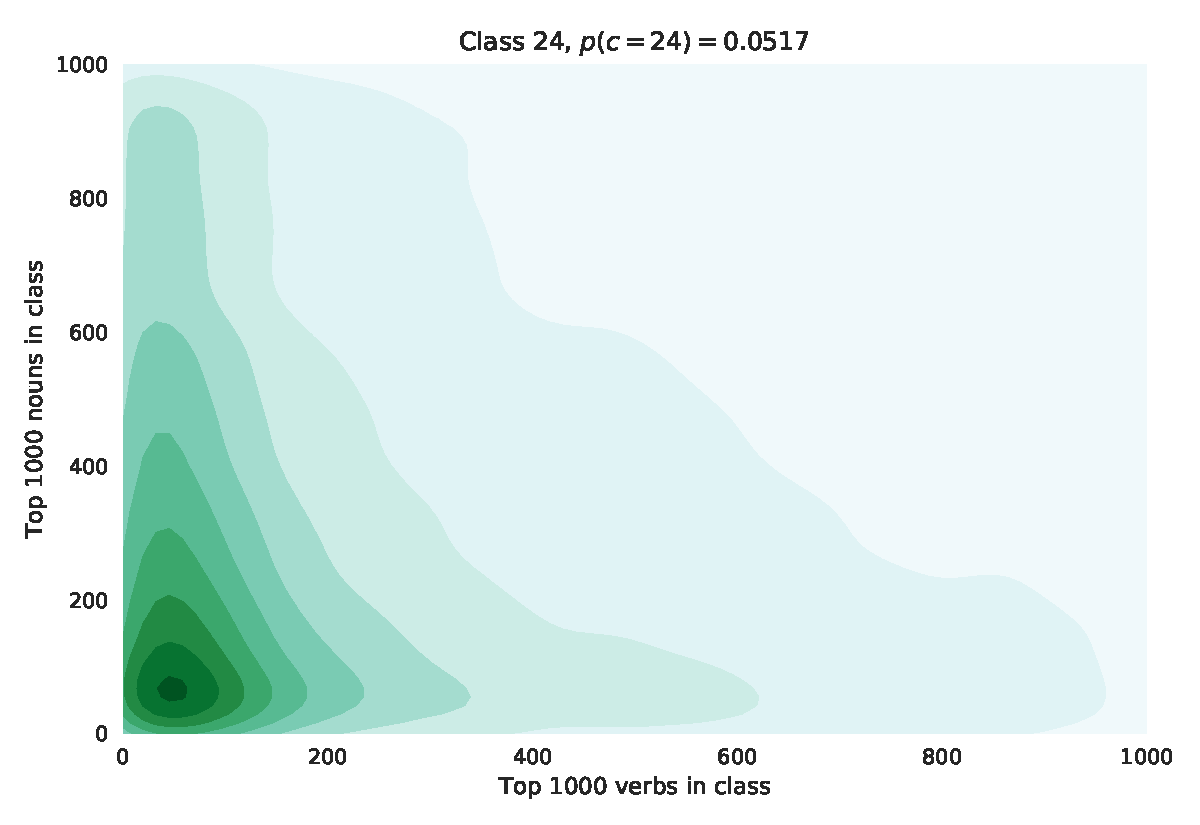
\includegraphics[width=\textwidth]{class_24.pdf}
  \end{subfigure}

  \caption{Kernel density estimate of scatter plot of top 1000 nouns
    and verbs in various classes. Darker colors represent that many pairs
    are present in the data set and lighter colors represent that little
    to none of the pairs are present in the data set. All classes show the
    pattern that pairs of high probability verbs and high probability
    nouns often occur in the data set (represented by a dark green blob in
    the lower left corner of each plot). These four classes were
    selected from a model trained with $K=30$ classes.} 
  \label{fig:kde}
\end{figure}

\begin{table}
  \centering
  \begin{tabular}{c c c c c c c c}
    \toprule
    Class 0 & & Class 6 & & Class 10 & & class 24 & \\
    \midrule
    verbs & nouns & verbs & nouns & verbs & nouns & verbs & nouns \\
    \midrule
    has      & which     & have   & you       & go         & whom           & have  & chance \\
    is       & that      & get    & we        & start      & rules          & had   & effect \\
    have     & it        & find   & they      & showed     & using          & has   & right \\
    had      & this      & see    & people    & give       & let            & gave  & time \\
    led      & system    & do     & children  & offer      & prices         & got   & idea \\
    was      & fact      & do     & one       & gives      & unit           & won   & one \\
    took     & the       & need   & that      & apply      & society        & get   & experience \\
    includes & much      & take   & god       & includes   & type           & give  & opportunity \\
    gives    & who       & know   & anyone    & carry      & principles     & see   & interest \\
    provides & one       & get    & women     & making     & manufacturers  & lost  & nothing \\
    \bottomrule
  \end{tabular}
  \caption{Top-10 verbs and nouns for class 0 and 6.}
  \label{table:top10}
  \end{table}

  Lastly, Table~\ref{table:topnoun} contains the top nouns for two
verbs based on the noun distribution inferred using the
sub-categorization model. For both nouns the top-class is
shown. Effectively this model only selects classes that are most
likely for each model, \ie, no new distribution over nouns is
induced. The probabilities shown in this table are $p(n|v)$ (and thus,
not class probabilities). A notable difference between the top-nouns
for these two verbs is that \textit{go} has much higher probabilities
for its top nouns than \textit{went}. The authors currently do not
have an explanation for this.

  \begin{table}
    \centering
\begin{tabular}{c c c c}
\toprule
go & class 18 & went & class 5 \\
noun & prob. & noun & prob \\
\midrule
i & 0.168        & shares & 0.002 \\
we & 0.035       & profits & 0.002 \\
we & 0.015       & earnings & 0.002 \\
they & 0.014     & sales & 0.002 \\
they & 0.005     & one & 0.002 \\
you & 0.004      & years & 0.001 \\
she & 0.003      & number & 0.001 \\
one & 0.002      & sun & 0.001 \\
people & 0.001   & year & 0.001 \\
one & 0.001      & prices & 0.001 \\
\bottomrule
\end{tabular}
\caption{Top-10 nouns for verb `go' and `went' for class 18 and class 5.}
\label{table:topnoun}
\end{table}

\section{Changing to VAE} % TODO change this title
In order to use the verb-noun pairs as an input for the VAE, the data first had to be converted to a vector input. Both the verb and noun from each pair are converted to a pretrained word2vec\cite{mikolov2013efficient} word embedding trained on the Google News Dataset\footnote{https://code.google.com/archive/p/word2vec/} and then concatenated. Pairs that contained words not in the pretrained model, were discarded from the dataset used for the VAE. To relationships between the verbs and nouns were represented as a one-hot encoded vector. To increase the reliability of learned model, we discarded all relations that were present in less than 2000 pairs, leaving 29 from the 324 different relations. From the 2,002,378 pairs in the original dataset, 1,818,740 were usable as an input for the VAE.  
% Convert verbs and nouns to word embeddings from google (word2vec ref / google )

% Relations with multihot

% Baseline by comparing the wordvector representation with t-sne

% Maybe start a new chapter here?
To visualize the clusters, each of the pair vector representations in the test set were plotted using t-sne and colored with their corresponding cluster. The exact same train and test set were used to train both the EM and VAE models. The results are shown in figure \fig{TODOFIXFIGURE}

\section{Conclusion} % Jorn & Bram
In this study, part of the results presented
in~\cite{rooth1999inducing} were reproduced. Similar results were
obtained, however, the results reported in~\cite{rooth1999inducing}
are not exactly reproduced. A probable cause for this is the different
methods of data acquisition (\ie, the difference in quality of the
parser). Moreover, an analysis was performed on the clusters obtained
and it was shown that the cluster behave as expected, that is,
probable nouns and verbs within a cluster also often occur in the data
set. Moreover, it was shown that apart from the high probability verbs
and nouns, there are cluster for nouns that occur often (with many
verbs) and vice versa. In sum, unsupervised methods may be highly
effective in inducing slot annotations and sub-categorizations,
however, a good train set is very important.

\bibliographystyle{plain}
\bibliography{ref}

\onecolumn
\appendix
\section{Slot Annotation Model Update Equation Derivation}
\label{sec:part1}
In this appendix, detailed derivations of the update equations for the
EM algorithm for the latent class model are presented. First the model
is described in detail in Section~\ref{sec:model}, followed by the
derivation of the update equations in Section~\ref{sec:em}.

\subsection{Model}
\label{sec:model}
Let $V = \{v_1, \ldots, v_{|V|}\}$ denote the set of verbs, $N =
\{n_1, \ldots, n_{|N|}\}$ the set of nouns and $C = \{c_1,\ldots,
c_K\}$ the set of classes. The data is provided as a set of 2-tuples
$\mathcal{Y} = \{(v_1, n_1), \ldots, (v_M, n_M)\}$ for $n \in N, v \in V$.  Then our
(complete) model is defined as:
\begin{align}
  p(C, \mathcal{Y}) &= \prod_{m=1}^{M}p(c_m)p(v_m|c_m)p(n_m|c_m) \\
             &= \prod_{m=1}^{M}
                \cat(c_m|\sigma_1, \ldots, \sigma_k)
                \cat(v_m|\phi_1^{(c_m)}, \ldots, \phi_{|V|}^{(c_m)})
                \cat(n_m|\lambda_1^{(c_m)}, \ldots, \lambda_{|N|}^{(c_m)}) \\
             &= \prod_{m=1}^{M}
                \prod_{k=1}^K \sigma_k^{[c_m=k]} 
                \prod_{i=1}^{|V|} {(\phi_i^{(c_m)})}^{[v_m=i]}
                \prod_{j=1}^{|N|} {(\lambda_j^{(c_m)})}^{[n_m=j]} \\
 \end{align}
 Hence, the log-likelihood is
 \begin{align}
   \log p(C, \mathcal{Y})
   &=
     \sum_{m=1}^{M}
     \sum_{k=1}^K [c_m = k]\log \sigma_k +
     \sum_{i=1}^{|V|} [v_m = i]\log \phi_i^{(c_m)} +
     \sum_{j=1}^{|N|} [n_m = j]\log \lambda_j^{(c_m)}
 \end{align}


\subsection{Expectation Maximization to Infer Unobserved Classes}
\label{sec:em}
In this section the update equations for the EM algorithm are derived.
For clarity, for the rest of this section, $\mathbb{E}_{p(C | n_m, v_m,
\thetaold)}[\cdot] \triangleq \mathbb{E}[\cdot]$, and $[\cdot]$
denotes the Iverson bracket.



\subsubsection{E-Step}
\label{sec:estep}
Following the EM algorithm~\cite{dempster1977maximum}, in the E-step the expectation of the
complete log-likelihood is evaluated under the conditional
distribution of the latent variables given the observed variables.  In
this specific case that results in:

\begin{align}
  \mathcal{Q}(\theta | \thetaold)
  &= \mathbb{E}_{p(C | \mathcal{Y}, \thetaold)} \left[ \log p(C, N, V | \theta) \right] \\
  &= \sum_{m=1}^{M} \mathbb{E} \left[ \log p(C, n_m, v_m | \theta) \right] \\
  &= \sum_{m=1}^{M} \mathbb{E} \left[ 
     \sum_{k=1}^K [C = k]\log \sigma_k +
     \sum_{i=1}^{|V|} [v_m = i]\log \phi_i^{(C)} +
     \sum_{j=1}^{|N|} [n_m = j]\log \lambda_j^{(C)}
 \right] \\
  &= \sum_{m=1}^{M} \left\{
     \sum_{k=1}^K \mathbb{E}\left[[C = k]\right]\log \sigma_k +
     \sum_{i=1}^{|V|} [v_m = i] \mathbb{E}\left[\log \phi_i^{(C)} \right] +
    \sum_{j=1}^{|N|} [n_m = j] \mathbb{E}\left[\log \lambda_j^{(C)} \right]
    \right\}.
\end{align}
To evaluate this function, we need compute the expectations in the
equation above, \ie:
\begin{align}
  \mathbb{E}\left[[C = k] \right] &= p(k|v_m, n_m) \\ 
  \mathbb{E}\left[ \log \phi_i^{(C)} \right] &= \sum_{k=1}^K p(k | v_m, n_m) \log \phi_i^{(k)} \\
  \mathbb{E}\left[ \log \lambda_j^{(C)} \right] &= \sum_{k=1}^K p(k | v_m, n_m) \log \lambda_j^{(k)}.
\end{align}
Hence, in the E-step only $p(k | v_m, n_m)$ is computed, for $k = 1, \ldots, K$
and $(v_m, n_m) \in \mathcal{Y}$, \textit{i.e.:}
\begin{align}
  p(c | v_m, n_m, \thetaold)
  &= \frac{p(c, v_m, n_m, \thetaold)}{\sum_{k=1}^K p(k, v_m, n_m | \thetaold)} \\
  &= \frac{\sigma^t_c \phi^{c,t}_{v_m} \lambda^{c,t}_{v_m} }
          {\sum_{k=1}^K \sigma^t_k \phi^{c,t}_{v_m} \lambda^{c,t}_{v_m} }
\end{align}

\subsubsection{M-step}
\label{sec:mstep}
In the M-step $\theta^{t+1} = \arg\max_\theta Q(\theta |
\thetaold)$ is computed. Here the derivation of the update equations
for each parameters $(\sigma, \phi, \lambda)$ is performed seperately.
Since the optimization is performed over constraint variables,
Lagrange multipliers\footnote{$\lambda$ is often used to denote the
Lagrange multiplier, but since $\lambda$ is already in use,
$\gamma$ is used here.} are introduced.
\begin{align}
  \mathcal{L}(\theta|\thetaold) = \mathcal{Q}(\theta|\thetaold)
  + \gamma^{(\sigma)} (1 - \sum_{k=1}^K \sigma_k)
  + \sum_{k=1}^{K} \gamma_k^{(\phi)} (1 - \sum_{v} \phi_v^{(k)})
  + \sum_{k=1}^{K} \gamma_k^{(\lambda)} (1 - \sum_{n} \lambda_n^{(k)})
 \end{align}
 Given this optimization objective, the update equations are easily
 obtained, \ie,
 \begin{align}
   \frac{\partial \mathcal{L}(\theta|\thetaold)}{\partial \lambda^k_n}
   &= \sum_{m=1}^M [n_m = n] \frac{\partial}{\partial \lambda_n^k}
      \mathbb{E}\left[ \log \lambda_n^{(C)} \right] - \gamma_k^{(\phi)} \\
   &= \sum_{m=1}^M [n_m = n] p(k|v_m, n_m, \thetaold) \frac{1}{\lambda_n^k} - \gamma_k^{(\phi)} = 0
%
\intertext{hence,}
%
     \lambda_n^k &= \frac{1}{\gamma_k^{(\phi)}} \sum_{m=1}^M [n_m = n] p(k|v_m, n_m, \thetaold)
                   \label{eq:lambda}
%
\intertext{Solve for $\gamma_k^{(\phi)}$ by summing both sides over $n$.}
%
                   1 &= \frac{1}{\gamma_k^{(\phi)}}
                        \sum_{m=1}^M \sum_{n=1}^{|N|} [n_m = n] p(k|v_m, n_m, \thetaold) \\
   \Rightarrow\quad \gamma_k^{(\phi)} &= \sum_{m=1}^M p(k|v_m, n_m, \thetaold) \label{eq:gammalambda}
%
\intertext{Now substitute~\eqref{eq:gammalambda} in~\eqref{eq:lambda} to obtain}
%
\lambda_n^{k,t+1} &= \frac{\sum_{m=1}^M [n_m = n] p(k|v_m, n_m, \thetaold)}
                   {\sum_{m=1}^M p(k|v_m, n_m, \thetaold)}
 \end{align}
 Note, this is the exact same update as presented in~\cite{rooth1999inducing},
 using a slightly different notation. The update for $\phi_v^k$ is similar in both result as
 derivation, hence the update equation is stated only:
 \begin{align}
\phi_v^{k,t+1} &= \frac{\sum_{m=1}^M [v_m = v] p(k|v_m, n_m, \thetaold)}
                   {\sum_{m=1}^M p(k|v_m, n_m, \thetaold)}
 \end{align}
 Lastly, the update equation for $\sigma_k$ is derived:
 \begin{align}
   \frac{\partial \mathcal{L}(\theta|\thetaold)}{\partial \sigma_k}
   &= \sum_{m=1}^M \mathbb{E}[[C = k]] \frac{1}{\sigma_k} - \gamma_\sigma \\ 
   &=  \sum_{m=1}^M p(k|v_m, n_m) - \gamma_\sigma= 0 \\
   \Rightarrow\quad \sigma_k
   &= \frac{1}{\gamma_\sigma}  \sum_{m=1}^M p(k|v_m, n_m) \label{eq:sigmak}
% 
\intertext{Sum both sides over $k$ to obtain}
% 
     \Rightarrow\quad 1 &= \frac{1}{\gamma_k} \sum_{m=1}^M \sum_{k=1}^K p(k, v_m, n_m) \\
                        &= \frac{M}{\gamma_\sigma} \\
     \Rightarrow\quad \gamma_\sigma &= M \label{eq:gammasigma} \\
   \intertext{Now substitute~\eqref{eq:gammasigma}
   into~\eqref{eq:sigmak} resulting in}
     \sigma_k^{t+1} &= \frac{1}{M} \sum_{m=1}^M p(k|v_m, n_m).
 \end{align}
 In sum, in the m-step phase of the EM algorithm the following updates are performed:
 \begin{align}
     \sigma_k^{t+1} &= \frac{1}{M} \sum_{m=1}^M p(k|v_m, n_m) \\
     \phi_v^{k,t+1} &= \frac{\sum_{m=1}^M [v_m = v] p(k|v_m, n_m, \thetaold)}
                     {\sum_{m=1}^M p(k|v_m, n_m, \thetaold)} \\
     \lambda_n^{k,t+1} &= \frac{\sum_{m=1}^M [n_m = n] p(k|v_m, n_m, \thetaold)}
                     {\sum_{m=1}^M p(k|v_m, n_m, \thetaold)}
 \end{align}
 for $k \in \{1, \ldots, K\}$, $v \in V$, and $n \in N$.

\end{document}
